\documentclass[journal]{IEEEtran}

\usepackage{cite}
\usepackage{amsmath,amssymb,amsfonts,amsthm,bm,mathtools}
\usepackage{graphicx}
\usepackage{booktabs,multirow,array}
\usepackage{algorithm}
\usepackage{algpseudocode}
\usepackage{url}
\usepackage{color}
\usepackage{balance}
\usepackage[hidelinks]{hyperref}

\graphicspath{{../figs/}}

\newtheorem{proposition}{Proposition}
\newtheorem{remark}{Remark}

\begin{document}

\title{EE-SE Pareto Boundary and Amplification Structure Optimization for Hybrid STAR-RIS}

\author{Hongjian Huang, Xiaonan Yang, and Renjie Liang%
\thanks{Corresponding author: Renjie Liang.}}
\maketitle

\begin{abstract}
Hybrid active-passive simultaneously transmitting and reflecting reconfigurable intelligent surfaces (STAR-RISs) can improve spectral efficiency (SE) relative to fully passive architectures, but their energy efficiency (EE) behavior remains insufficiently understood because existing analyses often rely on simplified amplifier-noise models, simplified control and switching power models, and asymmetric task models for the transmission and reflection sides. This paper develops a structured analytical framework for the EE-SE Pareto boundary of hybrid active-passive STAR-RISs. We first introduce a three-part power model that accounts for static controller and bias power, dynamic switching overhead, and communication-side transmit and amplification power. For a sparse active set, we derive a closed-form SE-optimal amplification structure and an active-on threshold that quantifies when amplification benefits outweigh amplifier noise. We then characterize the Pareto boundary via an $\epsilon$-constraint formulation with a low-complexity sparse-activation solver and show that the resulting coefficient rules extend across ES, TS, and SS modes. Numerical results under the simulated settings show that the proposed sparse-hybrid design improves EE over the considered baselines.
\end{abstract}

\begin{IEEEkeywords}
STAR-RIS, active RIS, hybrid active-passive RIS, energy efficiency, spectral efficiency, Pareto boundary, amplifier noise.
\end{IEEEkeywords}

\section{Introduction}
Simultaneously transmitting and reflecting reconfigurable intelligent surfaces (STAR-RISs) extend passive beam manipulation to simultaneous transmission and reflection, allowing a common surface to serve transmission-side and reflection-side users \cite{liu2021star,mu2022star}. This capability is attractive for asymmetric indoor-outdoor coverage, but purely passive STAR-RIS still suffers from multiplicative path loss.

Sparse active elements can mitigate this loss at the price of amplifier noise and hardware power \cite{ma2023activeee,peng2023hybrid,huang2024hybrid,zhang2022signal}. Measurement-driven studies further show that RIS power contains controller/bias and switching terms rather than a single constant \cite{wang2023static,wang2024practical}. These effects are more critical in STAR-RIS because the two sides compete for aperture, power split, and active hardware budget.

\begin{figure}[t]
	\centering
	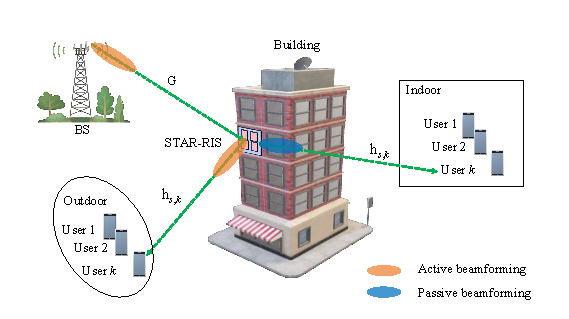
\includegraphics[width=\columnwidth]{systemEE3.pdf}
	\caption{\centering The hybrid STAR-RIS-aided wireless system.}
	\label{fig:system}
\end{figure}
Existing hybrid active-passive STAR-RIS studies still provide limited structural guidance on when to activate elements, how many to activate, and how to trade EE against SE across energy splitting (ES), time switching (TS), and space splitting (SS) \cite{vu2025hybridstar,zhu2025activepassive,soleymani2023starurlcc,zhang2024activestarisac}. To address this, we develop an equivalent formulation for hybrid STAR-RIS and derive tractable Pareto-boundary characterizations. The main contributions are as follows.
\begin{itemize}
    \item We formulate a hybrid active-passive STAR-RIS downlink and introduce a three-part power model with BS transmit power, controller/bias power, switching overhead, and amplification power.
    \item For a fixed active set, we derive an equivalent side-wise SINR model, a closed-form SE-optimal common gain, an explicit active-on threshold, and a power-minimizing scalar refinement with a sufficient convexity condition.
    \item We develop a sparse-activation $\epsilon$-constraint solver consistent with the analytical model and show that its coefficient rules extend across ES, TS, and SS; simulations reveal that passive STAR-RIS is competitive only at low SE, whereas sparse hybrid activation is preferable at moderate-to-high SE.
\end{itemize}

\section{System Model}
\subsection{Hybrid active-passive STAR-RIS downlink}
Consider a BS with $M$ antennas serving $K_t$ users on the transmission side and $K_r$ users on the reflection side via an $N$-element STAR-RIS. Let $\mathcal{K}_t=\{1,\ldots,K_t\}$ and $\mathcal{K}_r=\{1,\ldots,K_r\}$. Under the ES protocol, the $n$th STAR-RIS element uses transmission and reflection coefficients
\begin{equation}
\theta_{n,s}=\sqrt{\rho_{n,s}}\beta_{n,s}e^{j\phi_{n,s}},\qquad s\in\{t,r\},
\label{eq:theta}
\end{equation}
with $\rho_{n,t}+\rho_{n,r}=1$, $0\le \rho_{n,s}\le 1$, and $1\le \beta_{n,s}\le \beta_{\max}$. For passive elements, $\beta_{n,s}=1$; for active elements, $\beta_{n,s}>1$ on the assigned side. Let $\mathcal{A}_t$ and $\mathcal{A}_r$ denote the active-element sets for transmission and reflection, and let $\mathcal{A}=\mathcal{A}_t\cup\mathcal{A}_r$.

Denote by $\mathbf{G}\in\mathbb{C}^{N\times M}$ the BS-to-STAR-RIS channel, and by $\mathbf{h}_{s,k}\in\mathbb{C}^N$ the STAR-RIS-to-user channel on side $s$ for user $k$. The received signal of user $(s,k)$ is
\begin{equation}
y_{s,k}=\mathbf{h}_{s,k}^H\mathbf{\Theta}_s\mathbf{G}
\sum_{j\in\mathcal{K}_s}\mathbf{w}_{s,j}x_{s,j}
+\mathbf{h}_{s,k}^H\mathbf{n}_{a,s}+n_{s,k},
\label{eq:received}
\end{equation}
where $\mathbf{\Theta}_s=\mathrm{diag}(\theta_{1,s},\ldots,\theta_{N,s})$, $\mathbf{w}_{s,j}$ is the BS beamformer for user $(s,j)$, $x_{s,j}$ is the unit-power information symbol, $n_{s,k}\sim\mathcal{CN}(0,\sigma_0^2)$ is thermal noise, and $\mathbf{n}_{a,s}$ collects the amplifier noises of the active elements on side $s$. We model
\begin{equation}
\mathbf{n}_{a,s}\sim\mathcal{CN}(\mathbf{0},\mathbf{C}_{a,s}),\qquad
\mathbf{C}_{a,s}=\mathrm{diag}(c_{1,s},\ldots,c_{N,s}),
\label{eq:na_stat}
\end{equation}
where $c_{n,s}=\rho_{n,s}\beta_{n,s}^2\sigma_a^2$ for $n\in\mathcal{A}_s$ and $c_{n,s}=0$ otherwise. The SINR of user $(s,k)$ becomes
\begin{equation}
\gamma_{s,k}=
\frac{\left|\mathbf{h}_{s,k}^H\mathbf{\Theta}_s\mathbf{G}\mathbf{w}_{s,k}\right|^2}
{\sum_{j\neq k}\left|\mathbf{h}_{s,k}^H\mathbf{\Theta}_s\mathbf{G}\mathbf{w}_{s,j}\right|^2
+\sigma_{a,s,k}^2+\sigma_0^2},
\label{eq:sinr_full}
\end{equation}
where $\sigma_{a,s,k}^2=\mathbf{h}_{s,k}^H\mathbf{C}_{a,s}\mathbf{h}_{s,k}$ is the active-noise term seen at user $(s,k)$.

\subsection{Three-part power-consumption model}
Motivated by recent measurement-based RIS power studies \cite{wang2023static,wang2024practical}, we write the total consumed power as
\begin{equation}
\begin{aligned}
P_{\mathrm{tot}}
&=\frac{1}{\eta_{\mathrm{PA}}}
\sum_{s\in\{t,r\}}\sum_{k\in\mathcal{K}_s}\|\mathbf{w}_{s,k}\|^2
+P_{\mathrm{ctrl}}+P_{\mathrm{bias}}|\mathcal{A}|  \\
&\quad +f_u\!\left(P_{\mathrm{sw},0}+P_{\mathrm{sw},1}|\mathcal{A}|\right) \\
&\quad +\sum_{n\in\mathcal{A}_t}\mu_t(\beta_{n,t}^2-1)
+\sum_{n\in\mathcal{A}_r}\mu_r(\beta_{n,r}^2-1),
\end{aligned}
\label{eq:power_model}
\end{equation}
where the terms represent BS transmit power, controller and bias power, switching overhead, and amplification power.

\subsection{Structured equivalent formulation}
To obtain interpretable structure, we use a equivalent model with side-wise zero-forcing directions, phase alignment on the dominant cascaded paths, and a common gain $\beta_s$ for all active elements on side $s$. Let $g_n$ be the effective BS-to-element channel after zero-forcing projection, and let $h_{s,k,n}$ be the $n$th entry of $\mathbf{h}_{s,k}$. Define the equivalent coherent-gain quantity
\begin{equation}
u_{s,k,n} = |g_n|\,|h_{s,k,n}|.
\label{eq:un}
\end{equation}
Then the side-wise effective coherent term for user $(s,k)$ is
\begin{equation}
\psi_{s,k}(\beta_s)=
\sum_{n\in\mathcal{P}_s}\sqrt{\rho_s}u_{s,k,n}
+\beta_s\sum_{n\in\mathcal{A}_s}\sqrt{\rho_s}u_{s,k,n},
\label{eq:psi}
\end{equation}
where $\mathcal{P}_s=\{1,\ldots,N\}\setminus\mathcal{A}_s$ contains passive elements and those active only for the opposite side. The corresponding active-noise term is
\begin{equation}
\zeta_{s,k}(\beta_s)=\sigma_0^2+
\rho_s\beta_s^2\sigma_a^2
\sum_{n\in\mathcal{A}_s}|h_{s,k,n}|^2.
\label{eq:noise_exact}
\end{equation}
We further assume equal per-user rate splitting within each side, which captures side-wise asymmetric traffic demands but not arbitrary user-specific QoS.
The minimum sum transmit power needed to satisfy a side target rate $R_s$ under equal user-rate splitting is then
\begin{equation}
p_s^{\min}(\beta_s)=
\sum_{k\in\mathcal{K}_s}
\frac{(2^{R_s/K_s}-1)\zeta_{s,k}(\beta_s)}{\psi_{s,k}^2(\beta_s)}.
\label{eq:minsidepower}
\end{equation}

\section{Problem Formulation}
The sum spectral efficiency is
\begin{equation}
R_\Sigma = \sum_{s\in\{t,r\}}\sum_{k\in\mathcal{K}_s}\log_2(1+\gamma_{s,k}),
\label{eq:sumrate}
\end{equation}
and the system energy efficiency is
\begin{equation}
\mathrm{EE} = \frac{R_\Sigma}{P_{\mathrm{tot}}}\quad \text{(bit/J)}.
\label{eq:ee}
\end{equation}

The original EE-maximization problem can be written as
\begin{equation}
\begin{aligned}
\max_{\mathbf{W},\,\bm{\rho},\,\bm{\phi},\,\bm{\beta},\,\mathcal{A}}
\quad & \frac{R_\Sigma}{P_{\mathrm{tot}}} \\
\text{s.t.}\quad &
R_{s,k}\ge \bar{R}_{s,k},\ \forall s,k, \\
&
\sum_{s,k}\|\mathbf{w}_{s,k}\|^2 \le P_{\max}^{\mathrm{BS}},\\
&
1\le \beta_{n,s}\le \beta_{\max},\ \forall n\in\mathcal{A}_s,\\
&
\beta_{n,s}=1,\ \forall n\notin\mathcal{A}_s,\\
&
\rho_{n,t}+\rho_{n,r}=1,\ 0\le \rho_{n,s}\le 1,\\
&
\rho_{n,s}\beta_{n,s}^2\sigma_a^2 \le \Gamma_{n,s},\ \forall n,s,
\end{aligned}
\label{eq:P0}
\end{equation}
where $\Gamma_{n,s}$ is a maximum noise-injection or hardware-safety limit. Problem \eqref{eq:P0} is highly non-convex because the objective is fractional and the variables remain coupled through beamforming, STAR coefficients, active gains, and active-set selection.

To trace the EE-SE Pareto boundary, we adopt the $\epsilon$-constraint formulation
\begin{equation}
\begin{aligned}
\mathcal{P}(\epsilon):\quad
\min_{\mathbf{W},\,\bm{\rho},\,\bm{\phi},\,\bm{\beta},\,\mathcal{A}}
\quad & P_{\mathrm{tot}} \\
\text{s.t.}\quad &
R_\Sigma \ge \epsilon, \\
& \text{constraints of \eqref{eq:P0}.}
\end{aligned}
\label{eq:epsilon}
\end{equation}
Every feasible solution of \eqref{eq:epsilon} yields one Pareto-boundary point. We next exploit the model structure to derive transferable design rules.

\section{Optimal Structure of the Amplification Factors}
\subsection{Equivalent side-wise SINR law}
For a fixed active set, define
\begin{equation}
\begin{aligned}
a_s &= \min_k \sum_{n\in\mathcal{P}_s}\sqrt{\rho_s}u_{s,k,n},\\
b_s &= \min_k \sum_{n\in\mathcal{A}_s}\sqrt{\rho_s}u_{s,k,n},\\
c_s &= \sigma_0^2,\\
d_s &= \max_k \rho_s\sigma_a^2\sum_{n\in\mathcal{A}_s}|h_{s,k,n}|^2.
\end{aligned}
\label{eq:abcd}
\end{equation}
Here, $a_s$ and $b_s$ are the conservative worst-user coherent-gain aggregates from $\mathcal{P}_s$ and $\mathcal{A}_s$, while $c_s$ and $d_s$ denote the thermal-noise baseline and effective active-noise coefficient.
With average side power $\bar{p}_s$, a conservative worst-user SINR lower bound is
\begin{equation}
\underline{\gamma}_s(\beta_s)=
\frac{\bar{p}_s(a_s+b_s\beta_s)^2}{c_s+d_s\beta_s^2}.
\label{eq:surrogate}
\end{equation}
Equation \eqref{eq:surrogate} captures the key tradeoff: coherent signal grows linearly in $\beta_s$, whereas injected active noise grows quadratically.

\begin{proposition}\label{prop:se_optimal}
For fixed $(a_s,b_s,c_s,d_s)$ with $a_s>0$, $c_s>0$, and $d_s>0$, the function $\underline{\gamma}_s(\beta_s)$ in \eqref{eq:surrogate} is unimodal over $[1,\beta_{\max}]$, and its SE-optimal gain is
\begin{equation}
\beta_{s,\mathrm{SE}}^\star=
\left[\frac{b_sc_s}{a_sd_s}\right]_{[1,\beta_{\max}]},
\label{eq:beta_closed}
\end{equation}
where $[x]_{[l,u]}=\min\{u,\max\{l,x\}\}$.
\end{proposition}

\begin{IEEEproof}
Differentiating \eqref{eq:surrogate} gives
\begin{equation}
\frac{\mathrm{d}\underline{\gamma}_s}{\mathrm{d}\beta_s}=
\frac{2\bar{p}_s(a_s+b_s\beta_s)(b_sc_s-a_sd_s\beta_s)}{(c_s+d_s\beta_s^2)^2}.
\label{eq:surrogate_derivative}
\end{equation}
The derivative changes sign only once, at $\beta_s=b_sc_s/(a_sd_s)$, which proves unimodality and \eqref{eq:beta_closed}.
\end{IEEEproof}

A direct corollary of \eqref{eq:surrogate_derivative} is the \emph{active-on threshold}:
\begin{equation}
\left.\frac{\mathrm{d}\underline{\gamma}_s}{\mathrm{d}\beta_s}\right|_{\beta_s=1}>0
\iff b_sc_s>a_sd_s
\iff \frac{b_s}{a_s}>\frac{d_s}{c_s}.
\label{eq:threshold}
\end{equation}
Equation \eqref{eq:threshold} states when active mode is worthwhile: the coherent-gain increase must exceed the normalized amplifier-noise penalty. At high SNR (small effective $c_s$), the condition becomes harder to satisfy.

\subsection{Power-minimizing gain and a sufficient convexity condition}
For a target side rate $R_s$, based on (9) and (16), we define the cost as the minimum BS transmit power meeting the rate target plus the intrinsic power consumed by the active amplifiers:
\begin{equation}
\Psi_s(\beta_s)=
\frac{K_s(2^{R_s/K_s}-1)(c_s+d_s\beta_s^2)}{\eta_{\mathrm{PA}}(a_s+b_s\beta_s)^2}
+\mu_s|\mathcal{A}_s|(\beta_s^2-1).
\label{eq:side_cost}
\end{equation}
Its first derivative is
\begin{equation}
\Psi_s'(\beta_s)=
\frac{2K_s(2^{R_s/K_s}-1)(a_sd_s\beta_s-b_sc_s)}{\eta_{\mathrm{PA}}(a_s+b_s\beta_s)^3}
+2\mu_s|\mathcal{A}_s|\beta_s,
\label{eq:side_derivative}
\end{equation}
and its second derivative is
\begin{equation}
\begin{aligned}
\Psi_s''(\beta_s)
&=\frac{2K_s(2^{R_s/K_s}-1)}{\eta_{\mathrm{PA}}(a_s+b_s\beta_s)^4}
\Big(a_s^2d_s-2a_sb_sd_s\beta_s+3b_s^2c_s\Big) \\
&\quad +2\mu_s|\mathcal{A}_s|.
\end{aligned}
\label{eq:side_second}
\end{equation}

\begin{proposition}\label{prop:convexity}
Assume the mixed case $a_s>0$, $b_s>0$, and $d_s>0$. If
\begin{equation}
\beta_{\max}
\le
\frac{a_s^2d_s+3b_s^2c_s}{2a_sb_sd_s},
\label{eq:convexity_cond}
\end{equation}
then $\Psi_s(\beta_s)$ is strictly convex on $[1,\beta_{\max}]$. Consequently, the side-wise power-minimizing gain is unique and can be found by checking the two boundaries and the unique root of \eqref{eq:side_derivative}.
\end{proposition}

\begin{IEEEproof}
Under \eqref{eq:convexity_cond}, the bracketed term in \eqref{eq:side_second} is non-negative on $[1,\beta_{\max}]$ and, being affine in $\beta_s$, can vanish at most once. Hence $\Psi_s''(\beta_s)$ is non-negative everywhere and positive on every nontrivial subinterval, so $\Psi_s'(\beta_s)$ is strictly increasing and $\Psi_s(\beta_s)$ is strictly convex. The unique minimum is attained at an endpoint or at the unique root of \eqref{eq:side_derivative}.
\end{IEEEproof}

\begin{table}[t]
\centering
\caption{Case classification for the optimization of $\beta_s$}
\label{tab:beta_case_classification}
\small
\setlength{\tabcolsep}{4pt}
\begin{tabular}{@{}>{\raggedright\arraybackslash}p{0.23\linewidth} >{\raggedright\arraybackslash}p{0.27\linewidth} >{\raggedright\arraybackslash}p{0.38\linewidth}@{}}
\toprule
\textbf{Case} & \textbf{Condition} & \textbf{Conclusion} \\
\midrule
Fully passive & $|\mathcal{A}_s|=0$ & $b_s=d_s=0$; no active gain is to be optimized; set $\beta_s^\star=1$. \\[3pt]

Active-no-benefit degenerate case & $|\mathcal{A}_s|>0$, $a_s>0$, $b_s=0$ & $\Psi_s'(\beta_s)>0$; $\Psi_s(\beta_s)$ is strictly increasing ; set$\beta_s^\star=1$. \\[3pt]

Fully active & $|\mathcal{A}_s|>0$, $a_s=0$, $b_s>0$ & $\Psi_s''(\beta_s)>0$ ; $\Psi_s(\beta_s)$ is strictly convex and admits a unique minimizer. \\[3pt]

Mixed active-passive & $a_s>0$, $b_s>0$ & If $\beta_{\max}\le \frac{a_s^2d_s+3b_s^2c_s}{2a_sb_sd_s}$, then $\Psi_s(\beta_s)$ is strictly convex on $[1,\beta_{\max}]$ and the minimizer is unique. \\
\bottomrule
\end{tabular}
\end{table}

In the numerical study, we therefore set $\beta_s=1$ in the first two cases, solve the strictly convex scalar problem in the fully active case, and use \eqref{eq:beta_closed} with the refinement of Proposition~\ref{prop:convexity} in the mixed case.

\subsection{Extension of the coefficient rules to TS and SS}
Since ES is already covered by \eqref{eq:abcd}, for $p\in\{\mathrm{TS},\mathrm{SS}\}$ let $\mathcal{P}_s^{(p)}$ and $\mathcal{A}_s^{(p)}$ denote the passive and active support sets. Then
\begin{align*}
a_s^{(p)} &= \min_k \sum_{n\in\mathcal{P}_s^{(p)}} u_{s,k,n}, &
 b_s^{(p)} &= \min_k \sum_{n\in\mathcal{A}_s^{(p)}} u_{s,k,n},\\
c_s^{(p)} &= \sigma_0^2, &
d_s^{(p)} &= \max_k \sigma_a^2 \sum_{n\in\mathcal{A}_s^{(p)}} |h_{s,k,n}|^2.
\end{align*}
For TS, $\mathcal{P}_s^{(\mathrm{TS})}=\{1,\ldots,N\}\setminus\mathcal{A}_s$ and the effective target becomes $R_s/\tau_s$; for SS, $\mathcal{P}_s^{(\mathrm{SS})}=\mathcal{S}_s\setminus\mathcal{A}_s$ with $\mathcal{S}_t\cup\mathcal{S}_r=\{1,\ldots,N\}$. Thus \eqref{eq:threshold} applies after replacing $(a_s,b_s,c_s,d_s)$ by $(a_s^{(p)},b_s^{(p)},c_s^{(p)},d_s^{(p)})$.

\section{Sparse-Activation Pareto Boundary Algorithm}
\subsection{Outer sparse active-element selection}
The threshold law suggests activating elements with large coherent gain and small noise/hardware cost. For a candidate element $n\notin\mathcal{A}_s$, introduce a relaxed inclusion variable $x_{n,s}\in[0,1]$. For fixed $R_s$, $\beta_s$, and current aggregates $(a_s,b_s,c_s,d_s)$, define
\[
C_s=\frac{K_s(2^{R_s/K_s}-1)}{\eta_{\mathrm{PA}}},\qquad
\Delta u_{n,s}=\sqrt{\rho_s}|g_n|\min_k|h_{s,k,n}|.
\]
The exact increment of $d_s$ depends on the maximizing user after inserting element $n$; for ranking we use the surrogate
\[
\Delta d_{n,s}\approx \rho_s\sigma_a^2\overline{|h_{s,k,n}|^2},\qquad
\overline{|h_{s,k,n}|^2}\triangleq \frac{1}{K_s}\sum_{k\in\mathcal{K}_s}|h_{s,k,n}|^2.
\]
Under the same conservative surrogate used in \eqref{eq:surrogate}--\eqref{eq:side_cost}, the $n$-dependent part of the side cost is approximated by
\[
\begin{aligned}
\Psi_s(x_{n,s})
&\approx
C_s\frac{c_s+\beta_s^2(d_s+x_{n,s}\Delta d_{n,s})}
{\big(a_s+b_s\beta_s+(\beta_s-1)x_{n,s}\Delta u_{n,s}\big)^2} \\
&\quad +\mu_s(|\mathcal{A}_s|+x_{n,s})(\beta_s^2-1) \\
&\quad +x_{n,s}(P_{\mathrm{bias}}+f_uP_{\mathrm{sw},1}).
\end{aligned}
\]
Therefore, the first-order increment at $x_{n,s}=0$ is
\[
\begin{aligned}
\left.\frac{\partial \Psi_s}{\partial x_{n,s}}\right|_{x_{n,s}=0}
&=
-\kappa_{1,s}\Delta u_{n,s}
+\kappa_{2,s}\Delta d_{n,s} \\
&\quad +P_{\mathrm{bias}}+f_uP_{\mathrm{sw},1}
+\mu_s(\beta_s^2-1),
\end{aligned}
\]
where
\[
\kappa_{1,s}=
\frac{2C_s(c_s+d_s\beta_s^2)(\beta_s-1)}{(a_s+b_s\beta_s)^3},
\qquad
\kappa_{2,s}=
\frac{C_s\beta_s^2}{(a_s+b_s\beta_s)^2}.
\]
Hence first-order activation is beneficial whenever
\[
\frac{\kappa_{1,s}\Delta u_{n,s}}
{\kappa_{2,s}\Delta d_{n,s}+P_{\mathrm{bias}}+f_uP_{\mathrm{sw},1}+\mu_s(\beta_s^2-1)} > 1.
\]
Absorbing $\kappa_{1,s}$ and $\kappa_{2,s}$ into normalized weights yields the practical ranking score
\begin{equation}
\xi_{n,s}=
\frac{\omega_s\sqrt{\rho_s}|g_n|\min_k|h_{s,k,n}|}
{\lambda_1\rho_s\sigma_a^2\overline{|h_{s,k,n}|^2}
+\lambda_2(P_{\mathrm{bias}}+f_uP_{\mathrm{sw},1})},
\label{eq:score}
\end{equation}
where $\omega_s$ reflects the side demand and $\lambda_1,\lambda_2$ absorb the side-wise constants. In the simulations, $\omega_t=\alpha$, $\omega_r=1-\alpha$, $\lambda_1=\sigma_0^{-2}$, and $\lambda_2=(P_{\max}^{\mathrm{BS}})^{-1}$. Candidates are ranked by $\max_s\xi_{n,s}$, assigned to the maximizing side, and then re-evaluated through \eqref{eq:minsidepower}, \eqref{eq:side_cost}, and \eqref{eq:power_model}.

\subsection{Inner gain and rate-split update}
For a given active cardinality $L=|\mathcal{A}|$, we search over the 1-D rate split $R_t=\alpha\epsilon$ and $R_r=(1-\alpha)\epsilon$. After updating $\mathcal{A}_t$ and $\mathcal{A}_r$ via \eqref{eq:score}, we compute $(a_s,b_s,c_s,d_s)$ and update $\beta_s$ case by case: set $\beta_s=1$ if $|\mathcal{A}_s|=0$ or $b_s=0$, solve $\min_{\beta_s\in[1,\beta_{\max}]}\Psi_s(\beta_s)$ if $a_s=0$, and otherwise use \eqref{eq:beta_closed} or Proposition~\ref{prop:convexity}. The best feasible $(L,\alpha)$ minimizes \eqref{eq:power_model}.

\begin{algorithm}[t]
\caption{Sparse-Activation Solver}
\label{alg:solver}
\begin{algorithmic}[1]
\Require Target $\epsilon$, cap $\beta_{\max}$, grids $\mathcal{L}$ and $\mathcal{G}_\alpha$
\State Initialize best power as $+\infty$
\For{$L\in\mathcal{L}$}
    \For{$\alpha\in\mathcal{G}_\alpha$}
        \State Build $\mathcal{A}_t,\mathcal{A}_r$ using score \eqref{eq:score}
        \State Compute $(a_s,b_s,c_s,d_s)$ for $s\in\{t,r\}$
        \ForAll{$s\in\{t,r\}$}
            \If{$|\mathcal{A}_s|=0$ or $b_s=0$}
                \State Set $\beta_s\gets 1$
            \ElsIf{$a_s=0$}
                \State Minimize $\Psi_s(\beta_s)$ on $[1,\beta_{\max}]$
            \Else
                \State Update $\beta_s$ using \eqref{eq:beta_closed} or Proposition~\ref{prop:convexity}
            \EndIf
        \EndFor
        \State Compute the required BS power via \eqref{eq:minsidepower}
        \If{$R_\Sigma\ge \epsilon$ and all constraints hold}
            \State Evaluate $P_{\mathrm{tot}}$ from \eqref{eq:power_model}
            \State Keep the candidate with minimum $P_{\mathrm{tot}}$
        \EndIf
    \EndFor
\EndFor
\State \Return best feasible candidate
\end{algorithmic}
\end{algorithm}

\subsection{Convergence and complexity}
Algorithm~\ref{alg:solver} terminates in finitely many steps because $\mathcal{L}$ and $\mathcal{G}_\alpha$ are finite. With closed-form gain updates, the dominant per-boundary-point complexity is
\[
\mathcal{O}\!\left(|\mathcal{L}||\mathcal{G}_\alpha|
\big(N\log N + N(K_t+K_r)\big)\right),
\]
where the $N\log N$ term comes from ranking the candidate active elements; adding the scalar refinement of Proposition~\ref{prop:convexity} only introduces a multiplicative 1-D search factor.

\section{Numerical Results}
We consider a hybrid STAR-RIS with $N=24$ elements, $K_t=K_r=2$, Nakagami-$m$ fading, and the normalized parameters listed in Table~\ref{tab:params}. All curves average $100$ independent channel draws. Unless stated otherwise, the BS power budget is $5.0$ W, the ES coefficients are $\rho_t=0.55$ and $\rho_r=0.45$, the TS slot fractions are $\tau_t=0.55$ and $\tau_r=0.45$, and the gain cap is $\beta_{\max}=5$.

\begin{table}[t]
\caption{Simulation parameters}
\label{tab:params}
\centering
\footnotesize
\begin{tabular}{lc}
\toprule
Parameter & Value \\
\midrule
STAR-RIS elements $N$ & $24$ \\
Users $(K_t,K_r)$ & $(2,2)$ \\
Fading model & Nakagami-$m$ \\
Nakagami parameters $(m_{BR},m_{RU})$ & $(1.0,1.0)$ \\
ES coefficients $(\rho_t,\rho_r)$ & $(0.55,0.45)$ \\ 
TS slot fractions $(\tau_t,\tau_r)$ & $(0.55,0.45)$ \\
Noise std. $(\sigma_0,\sigma_a)$ & $(0.26,0.05)$ \\
Maximum active gain $\beta_{\max}$ & $5$ \\
BS power budget $P_{\max}^{\mathrm{BS}}$ & $5.0$ W \\
Static controller power $P_{\mathrm{ctrl}}$ & $0.12$ W \\
Bias power $P_{\mathrm{bias}}$ & $0.016$ W per element \\
Dynamic base and slope $(P_{\mathrm{sw},0},P_{\mathrm{sw},1})$ & $(0.01,0.006)$ W \\
Amplifier coefficient $\mu_t=\mu_r$ & $0.0025$ W \\
PA efficiency $\eta_{\mathrm{PA}}$ & $0.38$ \\
Monte Carlo trials & $100$ \\
\bottomrule
\end{tabular}
\end{table}

Fig.~\ref{fig:pareto} shows the EE-SE Pareto boundary. Passive STAR-RIS is competitive only at very low SE, whereas the fully active benchmark pays excessive amplification cost as the target SE increases. The proposed sparse-hybrid design dominates the medium-to-high-SE region and remains feasible up to $20$ bit/s/Hz. At $12$ bit/s/Hz, it improves EE by approximately 30.7\% over uniform hybrid activation, 74.9\% over the fully active design, and 94.4\% over the passive design.

\refstepcounter{figure}
\noindent\begin{minipage}{\columnwidth}
\centering
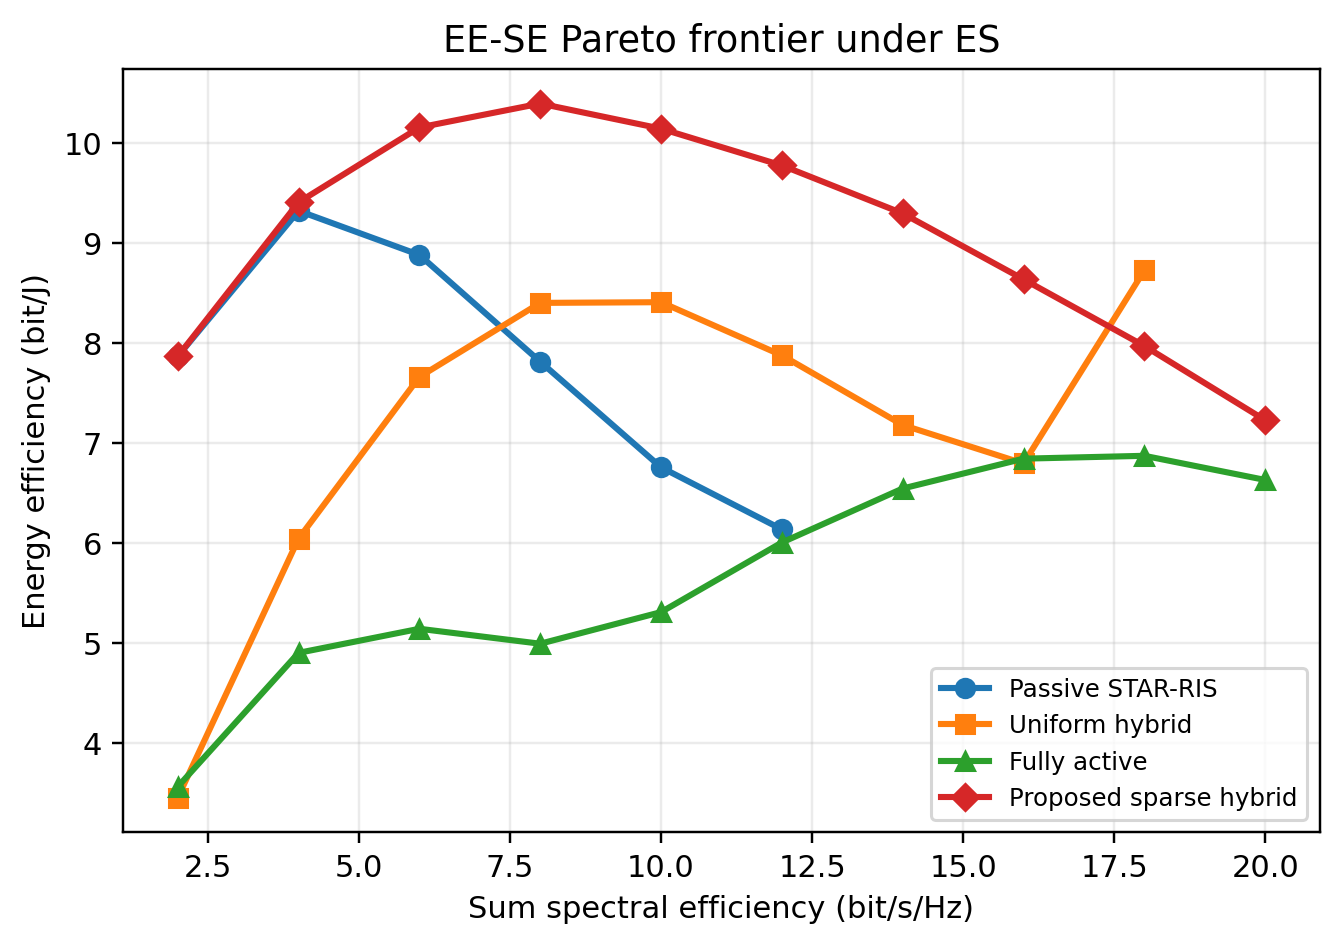
\includegraphics[width=\columnwidth]{fig_pareto_frontier.png}\\[2pt]
\footnotesize \textbf{Fig. \thefigure.} EE-SE Pareto boundary under ES.
\label{fig:pareto}
\end{minipage}\par\vspace{3pt}

Fig.~\ref{fig:design} compares the cross-mode design implications. TS requires the densest active set because the effective slot targets are inflated by $1/\tau_s$; at $12$ bit/s/Hz its active ratio is about $0.54$, versus about $0.27$ for ES and $0.29$ for SS. SS therefore tracks ES much more closely than TS in activation density. The gain curves show that SS stays near the gain cap, TS also uses high gains but with denser activation, and ES ramps more gradually before saturating.

\refstepcounter{figure}
\noindent\begin{minipage}{\columnwidth}
\centering
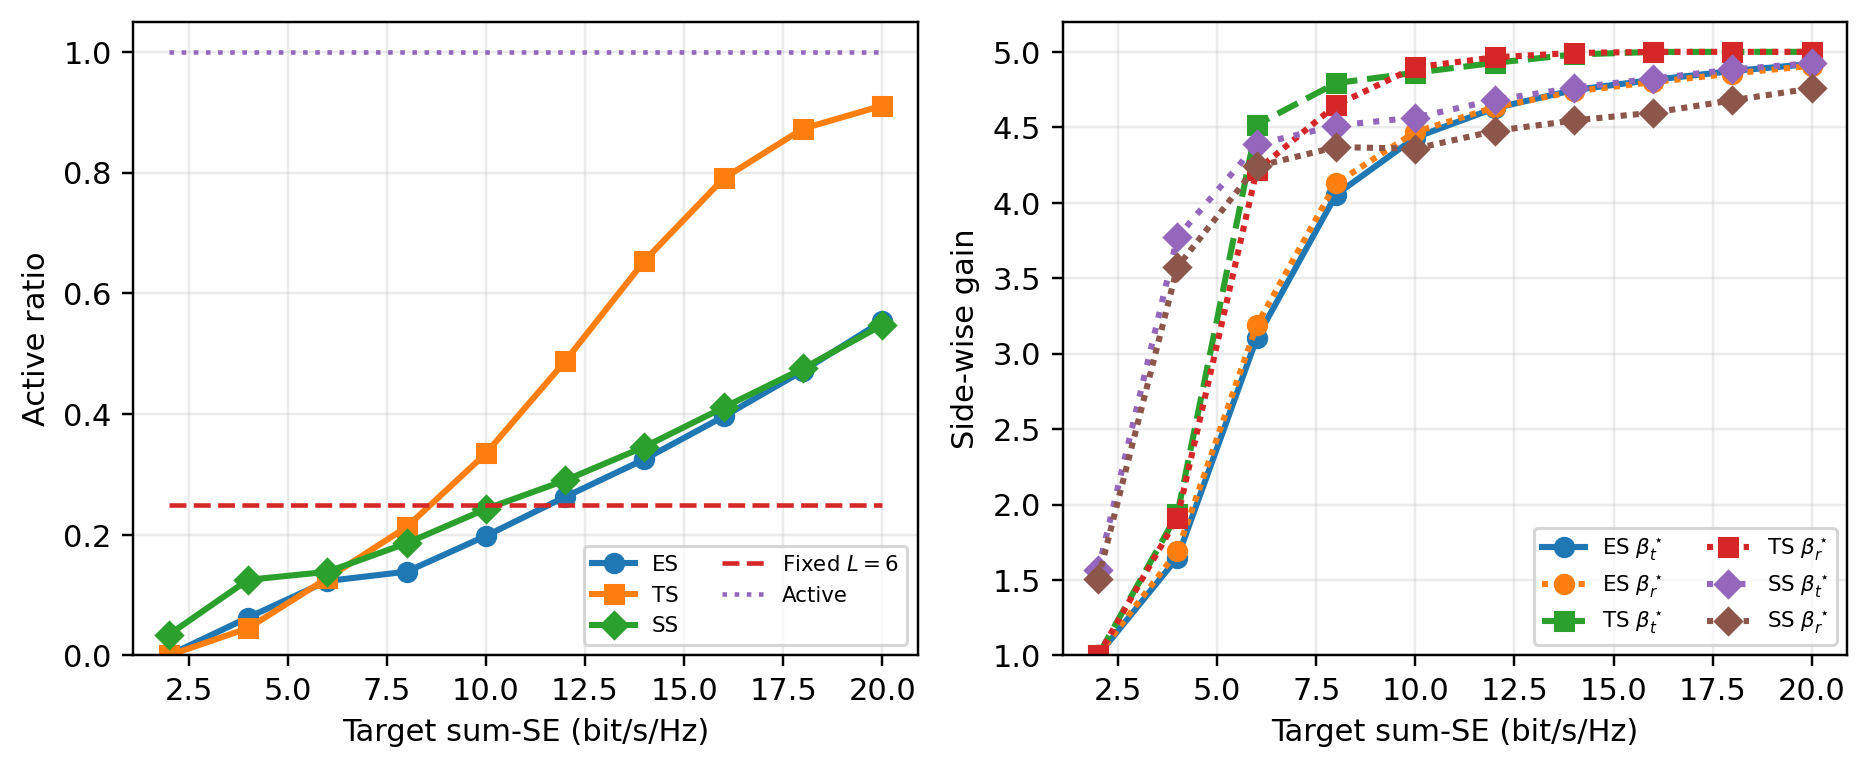
\includegraphics[width=\columnwidth]{fig_design_rules.png}\\[2pt]
\footnotesize \textbf{Fig. \thefigure.} Cross-mode design rules across ES, TS, and SS: (a) active ratio; (b) side-wise common gain.
\label{fig:design}
\end{minipage}\par\vspace{3pt}

Fig.~\ref{fig:noise_dyn} shows the hardware sensitivity across ES, TS, and SS at $R_\Sigma=12$ bit/s/Hz. In Fig.~\ref{fig:noise_dyn}(a), the average side-wise gain decreases with $\sigma_a$ for all three protocols, with the strongest drop under TS because slot-rate inflation already forces denser activation. In Fig.~\ref{fig:noise_dyn}(b), increasing the update frequency from $50$ Hz to $550$ Hz reduces EE for all three protocols; SS stays slightly above ES, whereas TS remains lower because its denser activation pattern magnifies the dynamic-cost penalty. The framework captures side-wise asymmetric rate demands through $(a_s,b_s,d_s)$ and the rate split $\alpha$; heterogeneous user-specific QoS and joint calibration/forwarding extensions are left for future work.

\refstepcounter{figure}
\noindent\begin{minipage}{\columnwidth}
\centering

\includegraphics[width=\columnwidth]{fig_noise_dynamic.png}\\[2pt]
\footnotesize \textbf{Fig. \thefigure.} Hardware sensitivity across ES, TS, and SS: (a) average side-wise gain versus amplifier noise; (b) EE versus switching overhead.
\label{fig:noise_dyn}
\end{minipage}\par\vspace{3pt}

Fig.~\ref{fig:breakdown} compares the ES power decomposition at $R_\Sigma=12$ bit/s/Hz. The fully active design minimizes the BS transmit-power share, about $0.38$ W on average, but pays excessive static/dynamic and amplification costs, with the amplification term alone reaching about $1.44$ W. The passive design avoids amplification but requires about $2.78$ W BS power. The proposed sparse-hybrid scheme achieves the lowest total power, about $1.44$ W versus about $1.91$ W for uniform hybrid, by sharply reducing the BS radiated-power requirement while keeping the amplification term well below the fully active benchmark.

\refstepcounter{figure}
\noindent\begin{minipage}{\columnwidth}
\centering

\includegraphics[width=\columnwidth]{fig_power_breakdown.png}\\[2pt]
\footnotesize \textbf{Fig. \thefigure.} Power breakdown at $R_\Sigma=12$ bit/s/Hz under ES.
\label{fig:breakdown}
\end{minipage}\par\vspace{3pt}

\section{Conclusion}
This paper studied the EE-SE tradeoff of hybrid active-passive STAR-RIS through a structured Pareto-boundary formulation linking amplifier noise, active-set sparsity, side-wise asymmetry, and hardware power. The analysis yielded a closed-form SE-optimal gain, an active-on threshold, and a sparse-activation rule, and the $\epsilon$-constraint solver translated them into a reproducible boundary generator. Numerical results showed that passive STAR-RIS is competitive only at low SE, whereas sparse hybrid activation is preferable at medium-to-high SE; TS requires denser activation and is more sensitive to amplifier noise than ES and SS, and robust CSI-imperfect or calibration-aware designs remain for future work.


\begin{thebibliography}{99}

%\bibitem{direnzo2020smart}
%M.~Di Renzo, A.~Zappone, M.~Debbah, M.-S. Alouini, C.~Yuen, J.~de Rosny, and S.~Tretyakov,
%``Smart radio environments empowered by reconfigurable intelligent surfaces: How it works, state of research, and the road ahead,''
%\emph{IEEE J. Sel. Areas Commun.}, vol.~38, no.~11, pp.~2450--2525, Nov.~2020.
%
%\bibitem{huang2019ee}
%C.~Huang, A.~Zappone, G.~C. Alexandropoulos, M.~Debbah, and C.~Yuen,
%``Reconfigurable intelligent surfaces for energy efficiency in wireless communication,''
%\emph{IEEE Trans. Wireless Commun.}, vol.~18, no.~8, pp.~4157--4170, Aug.~2019.
%
%\bibitem{wu2019irs}
%Q.~Wu and R.~Zhang,
%``Intelligent reflecting surface enhanced wireless network via joint active and passive beamforming,''
%\emph{IEEE Trans. Wireless Commun.}, vol.~18, no.~11, pp.~5394--5409, Nov.~2019.

%\bibitem{tang2020mimo}
%W.~Tang, M.~Z. Chen, X.~Chen, J.~Y. Dai, Y.~Han, M.~Di Renzo, Y.~Zeng, S.~Jin, Q.~Cheng, and T.~J. Cui,
%``MIMO transmission through reconfigurable intelligent surface: System design, analysis, and implementation,''
%\emph{IEEE J. Sel. Areas Commun.}, vol.~38, no.~11, pp.~2683--2699, Nov.~2020.

\bibitem{liu2021star}
Y.~Liu, X.~Mu, J.~Xu, D.~Niyato, R.~Schober, Y.~L. Guan, and C.~Yuen,
``STAR: Simultaneous transmission and reflection for 360-degree coverage by intelligent surfaces,''
\emph{IEEE Wireless Commun.}, vol.~28, no.~6, pp.~102--109, Dec.~2021.

\bibitem{mu2022star}
X.~Mu, Y.~Liu, L.~Guo, J.~Lin, and R.~Schober,
``Simultaneously transmitting and reflecting (STAR) RIS aided wireless communications,''
\emph{IEEE Trans. Wireless Commun.}, vol.~21, no.~5, pp.~3083--3098, May~2022.

\bibitem{ma2023activeee}
Y.~Ma, M.~Li, Y.~Liu, Q.~Wu, and Q.~Liu,
``Active reconfigurable intelligent surface for energy efficiency in MU-MISO systems,''
\emph{IEEE Trans. Veh. Technol.}, vol.~72, no.~3, pp.~4103--4107, Mar.~2023.

\bibitem{peng2023hybrid}
Q.~Peng, Q.~Wu, G.~Chen, R.~Liu, S.~Ma, and W.~Chen,
``Hybrid active-passive IRS assisted energy-efficient wireless communication,''
\emph{IEEE Commun. Lett.}, vol.~27, no.~8, pp.~2202--2206, Aug.~2023.

\bibitem{huang2024hybrid}
A.~Huang, X.~Mu, L.~Guo, and G.~Zhu,
``Hybrid active-passive RIS transmitter enabled energy-efficient multi-user communications,''
\emph{IEEE Trans. Wireless Commun.}, vol.~23, no.~9, pp.~10653--10666, Sep.~2024.

\bibitem{zhang2022signal}
Z.~Zhang, L.~Dai, X.~Chen, C.~Liu, F.~Yang, R.~Schober, and H.~V. Poor,
``Active RISs: Signal modeling, asymptotic analysis, and beamforming design,''
in \emph{Proc. IEEE GLOBECOM}, Rio de Janeiro, Brazil, 2022, pp.~1--6.

\bibitem{wang2023static}
J.~Wang, W.~Tang, S.~Jin, X.~Li, and M.~Matthaiou,
``Static power consumption modeling and measurement of reconfigurable intelligent surfaces,''
in \emph{Proc. EUSIPCO}, Helsinki, Finland, 2023, pp.~890--894.

\bibitem{wang2024practical}
J.~Wang, W.~Tang, J.~C. Liang, L.~Zhang, J.~Y. Dai, X.~Li, S.~Jin, Q.~Cheng, and T.~J. Cui,
``Reconfigurable intelligent surface: Power consumption modeling and practical measurement validation,''
\emph{IEEE Trans. Commun.}, vol.~72, no.~9, pp.~5720--5734, Sep.~2024, doi: 10.1109/TCOMM.2024.3382332.

\bibitem{vu2025hybridstar}
T.-H. Vu, T.~N. Nguyen, T.-T. Nguyen, and S.~Kim,
``Hybrid active-passive STAR-RIS-based NOMA systems: Energy/rate-reliability trade-offs and rate adaptation,''
\emph{IEEE Wireless Commun. Lett.}, vol.~14, no.~1, pp.~238--242, Jan.~2025.

\bibitem{zhu2025activepassive}
G.~Zhu, X.~Mu, L.~Guo, A.~Huang, and S.~Xu,
``STAR-RIS assisted SWIPT systems: Active or passive?''
\emph{IEEE Trans. Wireless Commun.}, vol.~25, pp.~4514--4529, 2026, doi: 10.1109/TWC.2025.3611793.

\bibitem{soleymani2023starurlcc}
M.~Soleymani, I.~Santamaria, and E.~A. Jorswieck,
``Spectral and energy efficiency maximization of MISO STAR-RIS-assisted URLLC systems,''
\emph{IEEE Access}, vol.~11, pp.~70833--70852, 2023.

\bibitem{zhang2024activestarisac}
S.~Zhang, W.~Hao, G.~Sun, C.~Huang, Z.~Zhu, X.~Li, and C.~Yuen,
``Joint beamforming optimization for active STAR-RIS-assisted ISAC systems,''
\emph{IEEE Trans. Wireless Commun.}, vol.~23, no.~11, pp.~15888--15902, Nov.~2024.

\end{thebibliography}

\end{document}
